\section{相关概念介绍}

\subsection{Android平台的蓝牙技术}
蓝牙(Bluetooth)是一种短距离无线通信标准,支持频率为2.4GHz左右的短距通信。Android平台一直以来都对蓝牙技术保持着良好的支持,使用一系列API可以在Android平台上实现简单的蓝牙操作。通过使用系统提供的BluetoothAdapter类和BluetoothDevice类,Android应用能够扫描附近的蓝牙设备、列出已经配对的蓝牙设备、建立RFCOMM通道、连接其他设备并传递数据\cite{androidbt}。在进行蓝牙连接前,在应用的Manifest文件中需要申请蓝牙控制权限。之后,使用BluetoothAdapter类中的方法可以开启蓝牙适配器并搜索设备,搜索到的设备将会返回其蓝牙地址,通过获取到的蓝牙地址就能建立连接。

在建立蓝牙连接后,使用BluetoothSocket类的方法可以建立作为客户端的连接。使用客户端方式连接的蓝牙设备可以收取服务器端设备传递的信息。通过验证UUID,两个设备能够正确建立连接。最终,使用InputStream类可以获取服务端传递的信息,该信息被存储在byte类型的变量中,并等待处理。Android平台蓝牙连接的过程可见图\ref{fig1}。

\begin{figure}[htbp]
\centering
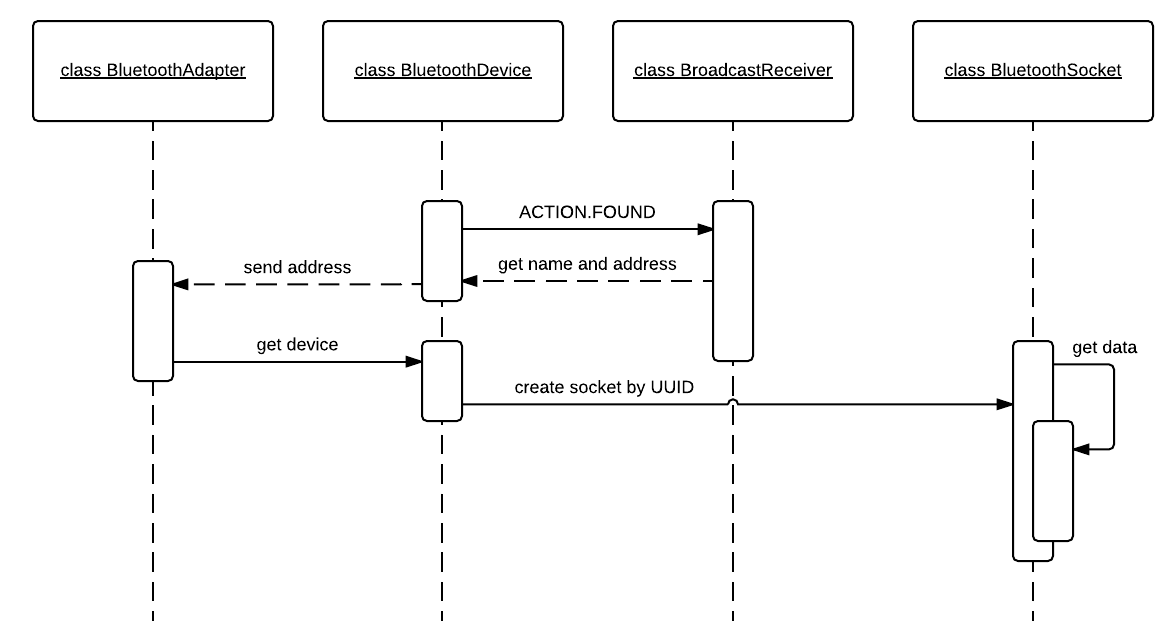
\includegraphics[width=0.9\columnwidth]{fig1.png}
\caption{
\label{fig1}
Android API蓝牙连接过程
}
\end{figure}

\subsection{ECG简介}

构成人体心脏肌肉的心肌细胞保持着细胞膜内外的离子浓度差异,因而造成了细胞膜内外存在电势差。记录这种电势差随细胞状态的变动,并将这种电活动曲线记录所得的图形被称为心电图(Electrocardiogram, ECG)。单个心肌细胞的膜内外电位变化过程可视为一对电偶的移动。如图\ref{fig2}所示,除极过程和复极过程的电位是相反的。因此,除极和复极过程所形成的电位变化波形方向相反,心电图因此包含正负两个方向的电位变化\cite{Diag}。

从整体来看,心脏电偶的位移局限在心肌内,可近似看作电偶固定在心脏中心,心脏中不同部位的心肌组织除极时间存在差异,从而造成了心脏电偶的方向变动。同时,电偶电力的强度也随心肌大小、薄厚的改变而改变。因此,将电极(被称为心电图的导联)放置在身体的不同位置时,检测到的心脏电偶变化是不同的。常规的导联体系包含肢导联和胸导联,不同的导联放置位置不同,代表的心脏状态也不同。在临床实践中通常综合12个导联的ECG波形来判断心脏状态。

\begin{figure}[htb]
\begin{center}
\begin{minipage}[b]{0.55\linewidth}
\begin{center}
  \subfigure[]{
  \begin{minipage}[b]{\textwidth}
  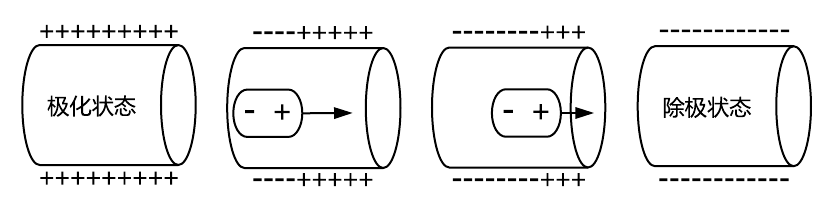
\includegraphics[width=\textwidth]{fig2a.png}
  
  \end{minipage}
  }
  \subfigure[]{
  \begin{minipage}[b]{\textwidth}
  
\includegraphics[width=\textwidth]{fig2b.png}
  \end{minipage}
  }
\end{center}
\end{minipage}
~~~~
\begin{minipage}[b]{0.4\linewidth}
  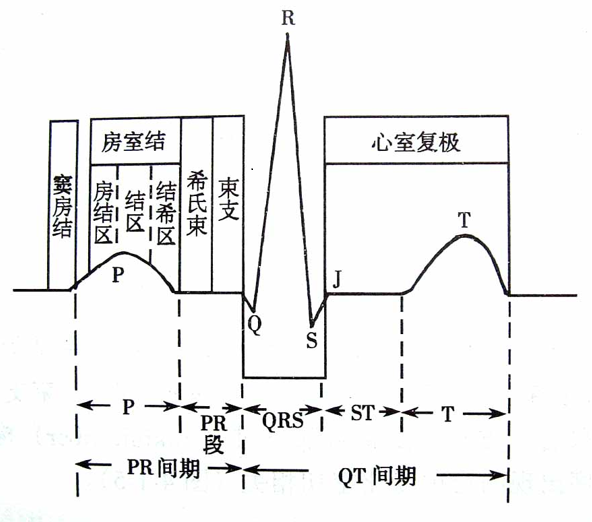
\includegraphics[width=0.9\textwidth]{fig3.png}  
\end{minipage}\\[-10pt]
\begin{minipage}[t]{0.55\linewidth}
\caption{\label{fig2}心肌细胞的除极与复极过程:(a)为除极过程,(b)为复极过程}
\end{minipage}
\begin{minipage}[t]{0.4\linewidth}
\caption{\label{fig3}ECG信号波形示意图}
\end{minipage}
\end{center}
\end{figure}

单幅的心电图通常包含P波、QRS波群和T波,这是根据波的大小和形态划分的(见图\ref{fig3})。通过观察一副ECG图像的PQRST波及其特点,能够了解心脏某部分或整体的搏动状况。在医学生的训练中,以下ECG图像特征的观察备受强调:
\begin{itemize}
\item 两个P波或R波的间隔时间(被称为PP间期或RR间期);
\item PP或RR间期的离散程度;
\item P波持续时间;
\item P波振幅;
\item P波与R波的间隔时间(被称为PR间期);
\item QRS波群的间隔时间(被称为QRS间期);
\item S波结束与T波开始之间的间隔时间(被称为ST段);
\item 经过矫正的QT间期(即$\mathrm{QT_c}$,可通过$\mathrm{QT_c = \frac{QT}{\sqrt{RR}}}$计算,其中QT表示实际QT间期,RR表示RR间期);
\end{itemize}

除此以外,还有一些基于波形形态的观测(如QRS波的主波方向)在诊断中也十分重要。这些波形形态能够反映心脏房室肥大情况、心肌缺血情况、心肌是否坏死等。
